\documentclass{beamer}
%
% Choose how your presentation looks.
%
% For more themes, color themes and font themes, see:
% http://deic.uab.es/~iblanes/beamer_gallery/index_by_theme.html
%
\mode<presentation>
{
  \usetheme{default}      % or try Darmstadt, Madrid, Warsaw, ...
  \usecolortheme{default} % or try albatross, beaver, crane, ...
  \usefonttheme{default}  % or try serif, structurebold, ...
  \setbeamertemplate{navigation symbols}{}
  \setbeamertemplate{caption}[numbered]
}

\usepackage[english]{babel}
\usepackage[utf8x]{inputenc}

\usepackage{amstext}
\usepackage{coloremoji}

\usepackage{graphicx}
\graphicspath{ {figs/} }

\setbeameroption{hide notes}
\setbeamertemplate{note page}[plain]
\usepackage{listings}
\usepackage{datetime}
\usepackage{url}

% specifications for presenter mode
%\beamerdefaultoverlayspecification{<+->}
%\setbeamercovered{transparent}

% math shorthand
\usepackage{bm}
\usepackage{amsmath}
\usepackage{mathtools}
\newcommand{\D}{\mathcal{D}}
\newcommand{\E}{\mathbb{E}}
\newcommand{\F}{\mathcal{F}}
\newcommand{\X}{\mathcal{X}}
\newcommand{\lik}{\mathcal{L}}
\DeclarePairedDelimiterX{\infdivx}[2]{(}{)}{%
  #1\;\delimsize\|\;#2%
}
\newcommand{\infdiv}{D\infdivx}
\DeclarePairedDelimiter{\norm}{\lVert}{\rVert}
\DeclareMathOperator*{\argmin}{arg\,min}
\DeclareMathOperator*{\argmax}{arg\,max}

% Bibliography
\usepackage{natbib}
\bibpunct{(}{)}{,}{a}{}{;}
\usepackage{bibentry}

%\nobibliography*
\title[lstmseq2seq]{``Sequence to Sequence Learning with \\ Neural Networks''
  \small (I.~Sutskever et al., 2014)}
\subtitle{\vspace*{0.5em} \scriptsize for the seminar \textit{Deep Time-Series
  Learning with Finance Applications},\\ organized by L.~El Ghaoui \&
  F.~Belletti, Fall 2017, UC Berkeley}
\author{Nima Hejazi}
\institute{Division of Biostatistics,\\ University of California, Berkeley}
\date{07 November 2017}

%%%%%%%%%%%%%%%%%%%%%%%%%%%%%%%%%%%%%%%%%%%%%%%%%%%%%%%%%%%%%%%%%%%%%%%%%%%%%%%%

\begin{document}

\begin{frame}
  \titlepage
\end{frame}

%%%%%%%%%%%%%%%%%%%%%%%%%%%%%%%%%%%%%%%%%%%%%%%%%%%%%%%%%%%%%%%%%%%%%%%%%%%%%%%%

\begin{frame}{Preview}

\begin{itemize}
  \itemsep10pt
  \item LSTM architecture solves sequence to sequence problems.
  \item RNNs are not sufficient since the dimensionality of the inputs and
    outputs needs to be known \textit{a priori} and fixed.
  \item Architecture: $2$ LSTMs --- (1) read input sequence, a single timestep
    at a time, to obtain fixed-dimensional vector representations, and (2)
    extract output sequence.
  \item Approach obtains a BLEU score of $34.81$ --- the best ever achieved by a
    neural net system.
  \item Use of deep LSTMs significantly outperformed that of shallow LSTMs, at a
    nearly negligible computational cost.
  \item \textbf{Key} finding: reversing the order of words in the input led to
    significantly better results.
\end{itemize}

\end{frame}

%%%%%%%%%%%%%%%%%%%%%%%%%%%%%%%%%%%%%%%%%%%%%%%%%%%%%%%%%%%%%%%%%%%%%%%%%%%%%%%%

\begin{frame}{The Data and Objective}

\begin{itemize}
  \itemsep10pt
  \item The WMT'$14$ English to French dataset was used.
  \item Models were trained on a ``selected'' subset of $12$M sentences,
    consisting of $348$M French words and $304$M English words.
  \item This translation task and the specific subset was chosen based on the
    availability of a tokenized training and test set and other benchmarks.
  \item A \textit{fixed} vocabulary was used for both languages --- that is, a
    set of $160,000$ of the most frequent words for the source language and
    $80,000$ for the target language were used.
\end{itemize}

\end{frame}

%%%%%%%%%%%%%%%%%%%%%%%%%%%%%%%%%%%%%%%%%%%%%%%%%%%%%%%%%%%%%%%%%%%%%%%%%%%%%%%%

\begin{frame}{The Model I: Recurrent Neural Networks}

\begin{itemize}
  \itemsep10pt
  \item RNNs are a straightforward generalization of feedforward neural networks
    for sequences.
  \item For a sequence of inputs $(x_1, \dots, x_T)$, an RNN computes a sequence
    of outputs $(y_1, \dots, y_T)$ by iterating over
    \begin{enumerate}
      \item $h_t = \text{sigm}(W^{hx}x_t + W^{hh}h_{t-1})$
      \item $y_t = W^{yh}h_t$
    \end{enumerate}
  \item Note from the above that it is not immediately clear how to apply this
    procedure over inputs and outputs of differing lengths --- in fact, such a
    procedure would \textbf{not} be simple.
  \item This problem is made even more severe when considering that inputs and
    outputs may have a complex and (very likely) non-monotonic relationship.
\end{itemize}

\end{frame}

%%%%%%%%%%%%%%%%%%%%%%%%%%%%%%%%%%%%%%%%%%%%%%%%%%%%%%%%%%%%%%%%%%%%%%%%%%%%%%%%

\begin{frame}{The Model II: Long Short-Term Memory Networks}

\begin{itemize}
  \itemsep10pt
  \item LSTMs overcome the problems faced by RNNs, providing a relatively simple
    way to learn in settings with long-range temporal dependencies.
  \item The LSTM operates by estimating $p(y_1, \dots, y_{T'} \mid x_1, \dots,
    x_T)$, where the lengths $T$ and $T'$ need not be identical.
  \item The approach here employed networks in two simple steps:
    \begin{enumerate}
      \item Obtain a fixed-dimensional representation $v$ of $(x_1, \dots, x_T)$
        (the last hidden state of the LSTM).
      \item Compute the probability of $y_1, \dots, y_{T'}$ by a standard
        LSTM-LM formulation:
        $$
        p(y_1, \dots, y_{T'} \mid x_1, \dots, x_T) = \prod_{t = 1}^{T'} p(y_t
          \mid v, y_1, \dots, y_{t-1}),
        $$
        where the distribution in the likelihood is represented by a softmax
        over all the words in the vocabulary.
    \end{enumerate}
\end{itemize}

\end{frame}

%%%%%%%%%%%%%%%%%%%%%%%%%%%%%%%%%%%%%%%%%%%%%%%%%%%%%%%%%%%%%%%%%%%%%%%%%%%%%%%%

\begin{frame}{The Model III: Long Short-Term Memory Architectures}

\begin{figure}[H]
  \centering
  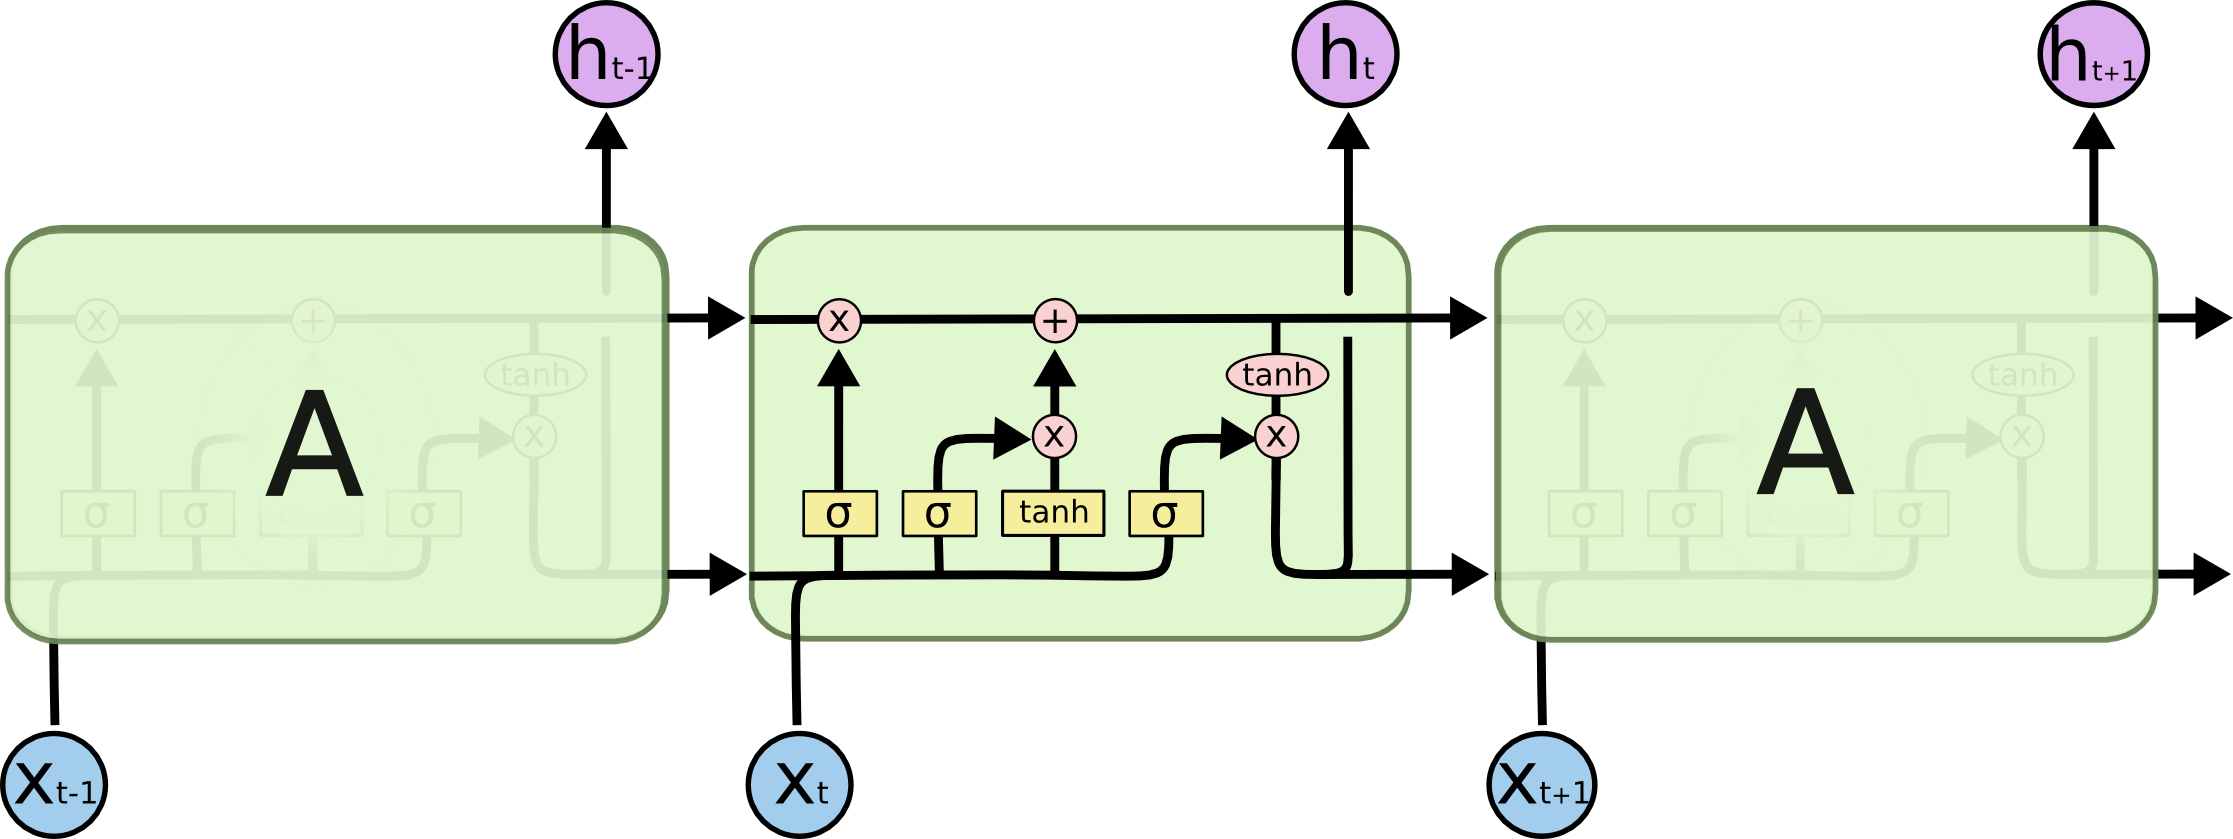
\includegraphics[width=\textwidth]{lstm-olah}
  \caption{There are $4$ interacting layers in the repeating module of an LSTM
    (source: C.~Olah's blog)}
\end{figure}

\end{frame}


%%%%%%%%%%%%%%%%%%%%%%%%%%%%%%%%%%%%%%%%%%%%%%%%%%%%%%%%%%%%%%%%%%%%%%%%%%%%%%%%

\begin{frame}{The Process I: Decoding and Rescoring}

\begin{itemize}
  \itemsep10pt
  \item The experiment centered on training a large LSTM on French-English
    sentence pairs, with training performed by maximizing the log-probability of
    a correct translation.
  \item The training objective, over a training set $\mathcal{S}$, was
    $$
     \frac{1}{\lVert \mathcal{S} \rVert} \sum_{(T,S) \in \mathcal{S}}
     \text{log} p(T \mid S)
    $$
  \item After training, the LSTM was used to produce translations:
    $$
     \hat{T} = \argmax_{T} p(T \mid S)
    $$
  \item Beam search is used to find the most likely translation. A beam of size
    $1$ gave good performance while a beam of size $2$ provided nearly the same
    utility as full beam search.
\end{itemize}

\end{frame}

%%%%%%%%%%%%%%%%%%%%%%%%%%%%%%%%%%%%%%%%%%%%%%%%%%%%%%%%%%%%%%%%%%%%%%%%%%%%%%%%

\begin{frame}{The Process II: Source Reversal}

\begin{itemize}
  \itemsep10pt
  \item A \textbf{key finding} of this work was that reversing source sentences
    (without reversing target sentences) provided great gains.
  \item Dropped LSTM perplexity (from $5.8$ to $4.7$), and improved test BLEU
    score from $25.9$ to $30.6$!
  \item Unfortunately, there is no ``complete explanation'' for this. 🤔
  \item How do such great gains arise from a simple manipulation?
    \begin{enumerate}
      \item The ``minimal time lag'' is lowered --- that is, when source and
        target sentences are concatenated, short-term dependencies are
        introduced (n.b., average distance remains unchanged).
      \item These can be exploited more easily by the LSTM. In fact, apparently,
        backpropagation has an easier time ``establishing communication'' under
        this sort of dependency structure.
      \item LSTMs exhibited better performance on long sentences, perhaps better
        memory utilization.
    \end{enumerate}
  \item ``The deepers'' got me here --- quite (read: too) empirical.
\end{itemize}

\end{frame}

%%%%%%%%%%%%%%%%%%%%%%%%%%%%%%%%%%%%%%%%%%%%%%%%%%%%%%%%%%%%%%%%%%%%%%%%%%%%%%%%

\begin{frame}{The Process III: Training the Model}

\begin{itemize}
  \itemsep10pt
  \item Used deep LSTMs with $4$ layers, $1000$ cells at each layer, and $1000$
    dimensional word embeddings (recall $v$ from before).
  \item Input vocab.: $160,000$ words; output vocab.: $80,000$ words.
  \item Deep LSTMs significantly outperformed shallow LSTMs, with each extra
    layer dropping model perplexity by nearly $10\%$.
  \item Mini-batches of size $128$ sequences were used for the gradient, and the
    problem of exploding gradients was avoided using ``clipping'':
    $s = \lVert g \rVert_{2}$ was computed (where $g$ is the gradient divided by
    minibatch size), and we set $g = 5 \cdot g / s$ if $s > 5$.
  \item Minibatches were set to have the same proportion of short and long
    sentences to help in training.
\end{itemize}

\end{frame}

%%%%%%%%%%%%%%%%%%%%%%%%%%%%%%%%%%%%%%%%%%%%%%%%%%%%%%%%%%%%%%%%%%%%%%%%%%%%%%%%

\begin{frame}{The Process IV: Parallelization}

\begin{itemize}
  \itemsep10pt
  \item A \textsc{C++} implementation on a single GPU processes $\sim 1700$
    words/second --- not fast enough!
  \item The aforementioned model was trained on a machine with $8$ GPUs, where
    each layer of the LSTM was executed on a different GPU, with activations
    communicated to the next GPU once complete.
  \item The remaining $4$ GPUs were used to compute the softmax, a matrix
    multiplication procedure involving a matrix of dimension $1000$ by $20000$.
  \item This parallelized architecture improved the speed of the implementation
    up to $6300$ words/second when minibatches of size $128$ were used ---
    training took $10$ days. 😞
\end{itemize}

\end{frame}

%%%%%%%%%%%%%%%%%%%%%%%%%%%%%%%%%%%%%%%%%%%%%%%%%%%%%%%%%%%%%%%%%%%%%%%%%%%%%%%%

\begin{frame}{Results I}

\begin{itemize}
  \itemsep10pt
  \item Surprisingly, good for long sentences as well as short ones.
  \item LSTM was \textit{sensitve} to the order of words in the sentence.
  \item LSTM was \textit{insensitive} to active versus passive voice.
  \item The best model trained was an ensemble of $5$ LSTMs, with a beam of size
    $12$, which achieved a BLEU score of $34.81$ (reducing the beam to size $2$
    gave a score of $34.50$).
  \item Rescoring of the baseline using the same ensemble of $5$ LSTMs produced
    a BLEU score of $36.5$ while the state of the art achieved $37.0$ (n.b.,
    the oracle score was $\sim 45$).
\end{itemize}

\end{frame}

%%%%%%%%%%%%%%%%%%%%%%%%%%%%%%%%%%%%%%%%%%%%%%%%%%%%%%%%%%%%%%%%%%%%%%%%%%%%%%%%

\begin{frame}{Results II}

\begin{figure}[H]
  \centering
  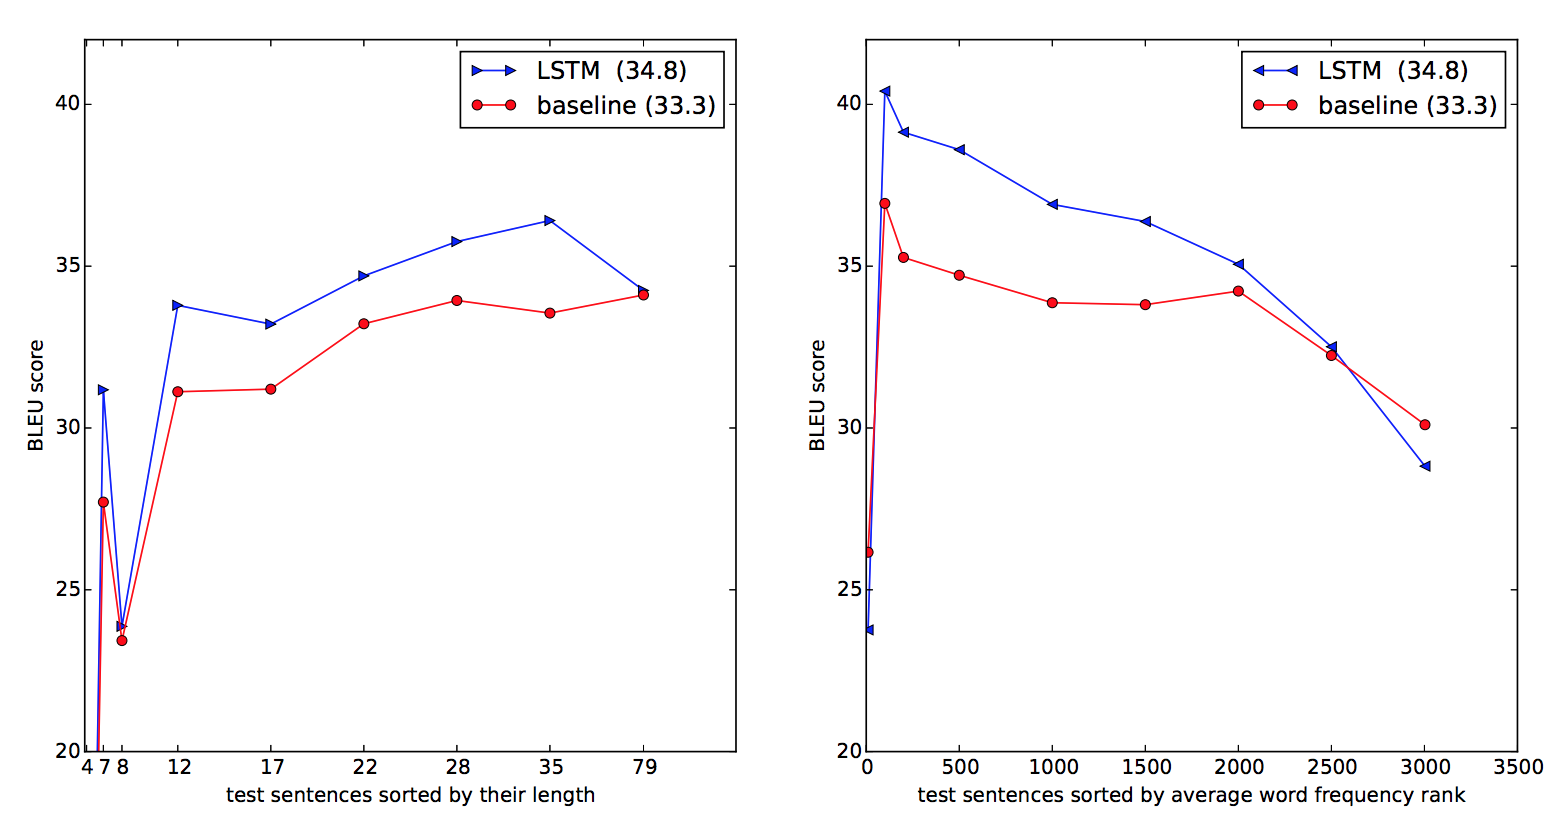
\includegraphics[scale=0.42]{performance-results}
  \caption{Performance of the LSTM model against the baseline (Figure 3 of
    Sutskever et al.)}
\end{figure}

\end{frame}

%%%%%%%%%%%%%%%%%%%%%%%%%%%%%%%%%%%%%%%%%%%%%%%%%%%%%%%%%%%%%%%%%%%%%%%%%%%%%%%%

\begin{frame}{Review}

\begin{itemize}
  \itemsep10pt
  \item LSTM architecture solves sequence to sequence problems.
  \item RNNs are not sufficient since the dimensionality of the inputs and
    outputs needs to be known \textit{a priori} and fixed.
  \item Architecture: $2$ LSTMs --- (1) read input sequence, a single timestep
    at a time, to obtain fixed-dimensional vector representations, and (2)
    extract output sequence.
  \item Approach obtains a BLEU score of $34.81$ --- the best ever achieved by a
    neural net system.
  \item Use of deep LSTMs significantly outperformed that of shallow LSTMs, at a
    nearly negligible computational cost.
  \item \textbf{Key} finding: reversing the order of words in the input led to
    significantly better results.
\end{itemize}

\end{frame}

%%%%%%%%%%%%%%%%%%%%%%%%%%%%%%%%%%%%%%%%%%%%%%%%%%%%%%%%%%%%%%%%%%%%%%%%%%%%%%%%

% don't want dimming with references
%\setbeamercovered{}
%\beamerdefaultoverlayspecification{}

\begin{frame}[c,allowframebreaks]{References}

\bibliographystyle{apalike}
\nocite{*}
\bibliography{refs}

\end{frame}

%%%%%%%%%%%%%%%%%%%%%%%%%%%%%%%%%%%%%%%%%%%%%%%%%%%%%%%%%%%%%%%%%%%%%%%%%%%%%%%%

\end{document}

